%%%%%%%%%%%%%%%%%%%%%%%%%%%%%%%%%%%%%%%%%%%%%%%%
% MAE 263F - Fall 2026 - SAMPLE Midterm 2
% 31 multiple-choice questions (the actual midterm has 20 x 0.5 pts = 10 pts), 100 minutes
% Covers the whole course except Chapter 12 (Neural ODE), emphasizing topics not on Midterm 1:
% plates and shells (Ch. 9, HW4), hydrodynamics (Ch. 10), contact (Ch. 11), time integration (Ch. 2, 3, 6), HW1-HW3.
% Solutions: SampleMidterm2_2026_solutions.tex
% Formatting follows Midterms/misc/Midterm 2026.tex and HW2_2026.tex
%
% HOW TO EDIT:
%   Each question is one \mcq{...} call on its own page (keeps the
%   Gradescope template aligned: one question per page).
%     \mcq{<question stem>}{<option a>}{<option b>}{<option c>}{<option d>}
%   NOTE: an option must not START with '[' (LaTeX reads it as an \item label);
%         wrap it in braces if needed, e.g. {{[0,1]} is correct}.
%   Write the answer key in the "% Answer:" comment under each question.
%   Figures go in figs/ (see \graphicspath) and can be placed inside the stem.
%%%%%%%%%%%%%%%%%%%%%%%%%%%%%%%%%%%%%%%%%%%%%%%%

\documentclass[letterpaper,11pt]{article}

%%%%%%%%%%%%%%%%%%%%%%%%%%%%%%%%%%%%%%%%%%%%%%%%
% Packages
%%%%%%%%%%%%%%%%%%%%%%%%%%%%%%%%%%%%%%%%%%%%%%%%
\usepackage[top = 2.5cm, bottom = 2.5cm, left = 2.5cm, right = 2.5cm]{geometry}
\usepackage[T1]{fontenc}
\usepackage[utf8]{inputenc}
\usepackage{graphicx}
\usepackage{setspace}
\setlength{\parindent}{0in}
\usepackage{float}
\usepackage{fancyhdr}
\usepackage{lastpage}
\usepackage{physics}
\usepackage{gensymb}
\usepackage{comment}
\usepackage{enumitem}
\usepackage{amsmath,amssymb,amsfonts}
\usepackage[dvipsnames]{xcolor}
\usepackage{tikz}
\input{glyphtounicode}
\pdfgentounicode=1
\usepackage{url}
\usepackage[hidelinks]{hyperref}

\graphicspath{{figs/}}

%%%%%%%%%%%%%%%%%%%%%%%%%%%%%%%%%%%%%%%%%%%%%%%%
% Header and footer
%%%%%%%%%%%%%%%%%%%%%%%%%%%%%%%%%%%%%%%%%%%%%%%%
\pagestyle{fancy}
\fancyhf{}
\lhead{\footnotesize MAE-263F Sample Midterm 2}
\rhead{\footnotesize \thepage \ of \pageref{LastPage}}
\lfoot{\footnotesize Copyright notice: Do not copy, distribute, republish, upload, post or transmit anything from the files hosted on the class website without written permission of the instructor}

%%%%%%%%%%%%%%%%%%%%%%%%%%%%%%%%%%%%%%%%%%%%%%%%
% Question macro
%   #1 = question stem, #2-#5 = options (a)-(d)
%   Each question starts on a new page, followed by blank space for work.
%   Students circle the letter of their answer directly in the list.
%%%%%%%%%%%%%%%%%%%%%%%%%%%%%%%%%%%%%%%%%%%%%%%%
\newcounter{qnum}
\newcommand{\qpts}{0.5}
\newcommand{\mcq}[5]{%
  \clearpage
  \stepcounter{qnum}%
  \section*{Question \theqnum \hfill \normalsize \qpts~pts}
  #1
  \begin{enumerate}[label=(\alph*)]
    \item #2
    \item #3
    \item #4
    \item #5
  \end{enumerate}
  \vspace{3mm}

  \textit{Space for work (not graded).}
}

%%%%%%%%%%%%%%%%%%%%%%%%%%%%%%%%%%%%%%%%%%%%%%%%
% Document
%%%%%%%%%%%%%%%%%%%%%%%%%%%%%%%%%%%%%%%%%%%%%%%%
\begin{document}

\thispagestyle{empty}

\begin{tabular}{p{15.5cm}}
{\large \bf Mechanics of Flexible Structures \& Soft Robots} \\
MAE-263F \\ Fall 2026 \\
\hline
\end{tabular}

\vspace*{0.3cm}

\begin{center}
    {\Huge \bf MAE-263F Sample Midterm 2} \\
    \vspace*{0.5cm}
    {\Large Fall 2026} \\
    \vspace*{0.5cm}
    {\Large Monday, November 23, 2026}
\end{center}

\vspace*{0.5cm}

{\Large \bf FULL NAME:} \underline{\hspace{10cm}} \\
\vspace*{0.3cm}

{\Large \bf UID:} \underline{\hspace{10cm}}\\
\vspace*{0.3cm}

{\Large \bf Time: 100 minutes (12:05 PM - 1:45 PM PST)}\\
\vspace*{0.3cm}

{\Large \bf Maximum points: 15.5} \quad (31 questions $\times$ 0.5 pts)\\
\textit{Note: This sample midterm has 31 problems. The actual midterm will have 20 problems, each worth 0.5 pts, for a maximum of 10 points.}

\vspace{0.3cm}

\noindent\fbox{%
    \parbox{\dimexpr\textwidth-2\fboxsep-2\fboxrule\relax}{%
        \small Please read the following instructions carefully:
        \begin{enumerate}[itemsep=1pt, topsep=3pt]
            \item This sample exam has 31 multiple-choice questions (the actual midterm has 20, each worth 0.5 pts). Each question is on its own page. For each question, \textbf{circle exactly ONE answer} (a, b, c, or d). \textbf{Only your a/b/c/d answer is graded.} Each question has space below it to show your work; \textbf{this work is NOT graded}.
            \item You are allowed to use a calculator (including scientific and graphing) for mathematical operations, including finding roots of polynomials. Computers and internet access are NOT allowed.
            \item This exam is open notes: you may bring ONE letter-sized two-sided cheat sheet and a printout of the course notes. You may write/type anything you wish on the cheat sheet.
            \item Once you are done, please use your phone to \textbf{scan your midterm and upload it to Gradescope} before leaving the exam hall. Do NOT write anything once the exam is over at 1:45 pm. However, you may scan and upload after 1:45 pm.
            \item Please make sure to \textbf{hand over the physical copy} of your midterm to the instructors.
            \item If you are unable to scan your exam, please inform the instructor/TA and simply hand over the physical copy.
        \end{enumerate}
    }%
}

\vspace{2ex}

\noindent\fbox{%
    \parbox{\dimexpr\textwidth-2\fboxsep-2\fboxrule\relax}{%
        \begin{center}
            \bf Honor Policy Statement
        \end{center}
        I agree to the UCLA student code of conduct for academic integrity. I affirm that I will not give or receive unauthorized help on this exam, and all work will be my own. I will not work on the exam outside the allowed time (12:05 pm - 1:45 pm PST).

        \vspace*{0.7cm}

        Signature: \underline{\hspace{5cm}} \hfill Date: \underline{\hspace{5cm}}
        \vspace*{0.2cm}
    }%
}

%%%%%%%%%%%%%%%%%%%%%%%%%%%%%%%%%%%%%%%%%%%%%%%%
% Questions
% All numerical answers were checked with Python (getTheta / gradEb_hessEb_Shell /
% getEdgesAndHinges for the shell questions); see the solutions file for the work.
%%%%%%%%%%%%%%%%%%%%%%%%%%%%%%%%%%%%%%%%%%%%%%%%

%%%%%%%%%%%%%%%%%%%%%%%%%%%%%%%%%%%%%%%%%%%%%%%%
% Shared problem setups (repeated on each page of a question set)
%%%%%%%%%%%%%%%%%%%%%%%%%%%%%%%%%%%%%%%%%%%%%%%%
\newcommand{\hingesetup}{The hinge has four nodes (in meters): $\mathbf{x}_0 = [0, 0, 0]$, $\mathbf{x}_1 = [2, 0, 0]$, $\mathbf{x}_2 = [1, 1, 0]$, and $\mathbf{x}_3 = [1, -1, -1]$, shown below. Write each node as $\mathbf{x}_k = [x_k, y_k, z_k]$. The hinge edge is $\mathbf{x}_0$--$\mathbf{x}_1$; triangle~1 is $(\mathbf{x}_0, \mathbf{x}_1, \mathbf{x}_2)$ and triangle~2 is $(\mathbf{x}_0, \mathbf{x}_1, \mathbf{x}_3)$. The triangle normals are $\mathbf{n}_0 = (\mathbf{x}_1 - \mathbf{x}_0) \times (\mathbf{x}_2 - \mathbf{x}_0)$ and $\mathbf{n}_1 = (\mathbf{x}_3 - \mathbf{x}_0) \times (\mathbf{x}_1 - \mathbf{x}_0)$.
\begin{center}
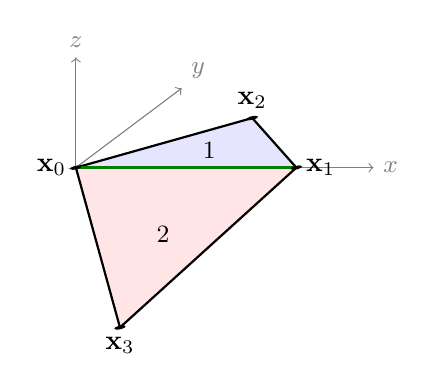
\begin{tikzpicture}[scale=1.4, x={(1cm,0cm)}, y={(0.6cm,0.45cm)}, z={(0cm,1cm)}]
  \draw[->, gray] (0,0,0) -- (2.7,0,0) node[right] {\small $x$};
  \draw[->, gray] (0,0,0) -- (0,1.6,0) node[above right] {\small $y$};
  \draw[->, gray] (0,0,0) -- (0,0,1.0) node[above] {\small $z$};
  \draw[thick, fill=blue!10] (0,0,0) -- (2,0,0) -- (1,1,0) -- cycle;
  \draw[thick, fill=red!10] (0,0,0) -- (2,0,0) -- (1,-1,-1) -- cycle;
  \draw[very thick, green!50!black] (0,0,0) -- (2,0,0);
  \foreach \p/\l/\a in {{(0,0,0)}/{\mathbf{x}_0}/left, {(2,0,0)}/{\mathbf{x}_1}/right, {(1,1,0)}/{\mathbf{x}_2}/above, {(1,-1,-1)}/{\mathbf{x}_3}/below} {
    \fill \p circle (0.045); \node[\a] at \p {$\l$};
  }
  \node at (1,0.35,0) {\small 1};
  \node at (1,-0.35,-0.45) {\small 2};
\end{tikzpicture}
\end{center}
}

%
% Question 1
% Source: HW4 Q1; Ch. 9.1 (edges and hinges)
%
\mcq{A rectangular plate with $4 \times 3$ nodes is meshed with 12 triangles as shown below (each square is cut by the diagonal from its lower-left to its upper-right corner).
\begin{center}
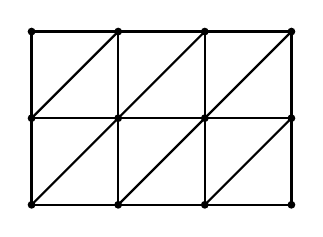
\begin{tikzpicture}[scale=1.1]
  \foreach \j in {0,1,2} { \draw[thick] (0,\j) -- (3,\j); }
  \foreach \i in {0,1,2,3} { \draw[thick] (\i,0) -- (\i,2); }
  \foreach \i in {0,1,2} { \foreach \j in {0,1} { \draw[thick] (\i,\j) -- (\i+1,\j+1); } }
  \foreach \i in {0,1,2,3} { \foreach \j in {0,1,2} { \fill (\i,\j) circle (0.045); } }
\end{tikzpicture}
\end{center}
How many edges and how many hinges does the mesh have?}
  {23 edges and 23 hinges}
  {17 edges and 7 hinges}
  {23 edges and 13 hinges}
  {26 edges and 13 hinges}
% Answer: (c). Edges: 9 horizontal + 8 vertical + 6 diagonal = 23. Boundary edges: 2(3+2) = 10. Hinges = 23 - 10 = 13. Checked with getEdgesAndHinges.

%
% Question 2
% Source: HW4 Q2; Ch. 9.1 (normals)
%
\mcq{Consider the following hinge. \hingesetup{}Compute the triangle normals $\mathbf{n}_0$ and $\mathbf{n}_1$.}
  {$\mathbf{n}_0 = [0, 0, 2]$, \ $\mathbf{n}_1 = [0, 2, -2]$}
  {$\mathbf{n}_0 = [0, 0, 2]$, \ $\mathbf{n}_1 = [0, -2, 2]$}
  {$\mathbf{n}_0 = [0, 0, 1]$, \ $\mathbf{n}_1 = [0, -1, -1]$}
  {$\mathbf{n}_0 = [2, 0, 0]$, \ $\mathbf{n}_1 = [0, -2, 2]$}
% Answer: (b). n0 = [2,0,0] x [1,1,0] = [0,0,2]; n1 = [1,-1,-1] x [2,0,0] = [0,-2,2]. (a) reverses the order of the cross product for n1.

%
% Question 3
% Source: HW4 Q2; Ch. 9.1 (signed hinge angle)
%
\mcq{Consider the same hinge as in Question~2 (repeated here). \hingesetup{}The hinge angle $\theta$ is the signed angle from $\mathbf{n}_0$ to $\mathbf{n}_1$ about the hinge vector $\mathbf{e}^0 = \mathbf{x}_1 - \mathbf{x}_0$: it is positive if $\mathbf{n}_0 \times \mathbf{n}_1$ points along $\mathbf{e}^0$ and negative otherwise. What is $\theta$?}
  {$-\pi/4$}
  {$\pi/2$}
  {$3\pi/4$}
  {$\pi/4$}
% Answer: (d). cos = n0.n1/(|n0||n1|) = 4/(2*2sqrt2) = 1/sqrt2 -> pi/4. n0 x n1 = [4,0,0] along +e0 -> +pi/4.

%
% Question 4
% Source: HW4 Q2-3; Ch. 9.2-9.3 (plate vs. shell energy)
%
\mcq{Consider the same hinge as in Questions~2--3 (repeated here), whose hinge angle is $\theta = \pi/4$. \hingesetup{}The bending stiffness is $k_b = 2\,\mathrm{N\,m}$ and the bending energy is $E_b = \frac{1}{2} k_b (\theta - \bar{\theta})^2$. What is $E_b$ if the hinge is a \emph{plate} ($\bar{\theta} = 0$), and if it is a \emph{shell} with $\bar{\theta} = \pi/6$?}
  {Plate: $\pi^2/8\,\mathrm{J}$; shell: $\pi^2/72\,\mathrm{J}$}
  {Plate: $\pi^2/16\,\mathrm{J}$; shell: $25\pi^2/144\,\mathrm{J}$}
  {Plate: $\pi^2/16\,\mathrm{J}$; shell: $\pi^2/144\,\mathrm{J}$}
  {Plate: $\pi/4\,\mathrm{J}$; shell: $\pi/12\,\mathrm{J}$}
% Answer: (c). Plate: 0.5*2*(pi/4)^2 = pi^2/16. Shell: (pi/4 - pi/6)^2 = (pi/12)^2 = pi^2/144. (a) drops 1/2; (b) uses theta + thetaBar; (d) does not square.

%
% Question 5
% Source: HW4 Q3-6 (energy after moving a node)
%
\mcq{Consider a setup similar to Question~4 (repeated here): a \emph{plate} ($\bar{\theta} = 0$) with $k_b = 2\,\mathrm{N\,m}$ and $E_b = \frac{1}{2} k_b \theta^2$. \hingesetup{}Node $\mathbf{x}_3$ is now moved from $[1, -1, -1]$ to $[1, 0, -1]$, and all other nodes stay where they are. What is the new bending energy $E_b$?}
  {$\pi^2/4\,\mathrm{J}$}
  {$0$}
  {$\pi^2/16\,\mathrm{J}$}
  {$\pi^2/2\,\mathrm{J}$}
% Answer: (a). n1 = [1,0,-1] x [2,0,0] = [0,-2,0]; perpendicular to n0 = [0,0,2]; n0 x n1 = [4,0,0] -> theta = +pi/2. E = 0.5*2*(pi/2)^2 = pi^2/4. (c) is the old energy; (d) drops 1/2.

%
% Question 6
% Source: HW4 Q3-5, Q8 (zero gradient components)
%
\mcq{Consider the same hinge as in Questions~2--4 (repeated here), as a plate with $E_b = \frac{1}{2} k_b \theta^2$. \hingesetup{}Which component of the gradient of the bending energy is \textbf{zero}?}
  {$\partial E_b / \partial y_3$}
  {$\partial E_b / \partial z_0$}
  {$\partial E_b / \partial z_2$}
  {$\partial E_b / \partial y_2$}
% Answer: (d). x2 lies in the plane z = 0 of triangle 1; moving it in x or y keeps n0's direction and does not affect n1, so theta and E_b do not change: dE/dy2 = 0. The others are nonzero (dF = [0,-0.39,1.18 | 0,-0.39,1.18 | 0,0,-1.57 | 0,0.79,-0.79]).

%
% Question 7
% Source: HW4 Q7 (finite-difference Jacobian)
%
\mcq{Let $\mathbf{f}(x, y) = \begin{bmatrix} f_1 \\ f_2 \end{bmatrix} = \begin{bmatrix} x^2 + 3y \\ x y^2 \end{bmatrix}$. At $(x, y) = (1, 1)$, estimate the Jacobian $J_{ij} = \partial f_i / \partial q_j$ (with $q_1 = x$, $q_2 = y$) using the forward finite difference \[ \frac{\partial f_i}{\partial q_j} \approx \frac{f_i(\mathbf{q} + \Delta q\, \mathbf{e}_j) - f_i(\mathbf{q})}{\Delta q}, \] where $\mathbf{e}_j$ perturbs only $q_j$, with $\Delta q = 0.1$. That is, perturb $x$ to $1.1$ (keeping $y = 1$) for the first column, and perturb $y$ to $1.1$ (keeping $x = 1$) for the second column. What is the finite-difference estimate of $\mathbf{J}$?}
  {$\begin{bmatrix} 2 & 3 \\ 1 & 2 \end{bmatrix}$}
  {$\begin{bmatrix} 2.1 & 1 \\ 3 & 2.1 \end{bmatrix}$}
  {$\begin{bmatrix} 0.21 & 0.3 \\ 0.1 & 0.21 \end{bmatrix}$}
  {$\begin{bmatrix} 2.1 & 3 \\ 1 & 2.1 \end{bmatrix}$}
% Answer: (d). f(1,1) = [4, 1]; f(1.1,1) = [4.21, 1.1] -> column 1 = [2.1, 1]; f(1,1.1) = [4.3, 1.21] -> column 2 = [3, 2.1]. (a) is the exact Jacobian, not the FD estimate; (b) is the transpose; (c) forgets to divide by eps.

%
% Question 8
% Source: Ch. 9.2 (stretching energy of a plate edge)
%
\mcq{An edge of a plate has undeformed length $l = 0.1\,\mathrm{m}$. The plate has Young's modulus $Y = 1\,\mathrm{MPa}$ and thickness $h = 1\,\mathrm{mm}$, so $k_s = \frac{\sqrt{3}}{2} Y h l^2 = 5\sqrt{3}\,\mathrm{N\,m}$. The edge is stretched to a length of $0.11\,\mathrm{m}$. What is its stretching energy $E_s = \frac{1}{2} k_s \left( \frac{\|\mathbf{e}\|}{l} - 1 \right)^2$?}
  {$\sqrt{3}/20\,\mathrm{J}$}
  {$\sqrt{3}/40\,\mathrm{J}$}
  {$\sqrt{3}/4\,\mathrm{J}$}
  {$\sqrt{3}/4000\,\mathrm{J}$}
% Answer: (b). Strain = 0.11/0.1 - 1 = 0.1; E = 0.5 * 5 sqrt3 * 0.01 = sqrt3/40 J. (a) drops 1/2; (c) does not square the strain; (d) uses the change in length (0.01 m) as the strain.

%
% Question 9
% Source: Ch. 9.2 (stiffness scaling with thickness)
%
\mcq{The thickness $h$ of a plate is doubled. By what factors do the bending stiffness $k_b = \frac{2}{\sqrt{3}} \frac{Y h^3}{12}$ and the stretching stiffness $k_s = \frac{\sqrt{3}}{2} Y h l^2$ change?}
  {Both double.}
  {Both increase by a factor of 8.}
  {$k_b$ doubles; $k_s$ increases by a factor of 8.}
  {$k_b$ increases by a factor of 8; $k_s$ doubles.}
% Answer: (d). kb ~ h^3 (x8), ks ~ h (x2). Thin plates bend much more easily than they stretch.

%
% Question 10
% Source: Ch. 9.1, 9.5; HW4 (sizes)
%
\mcq{A discrete plate has $N$ nodes. How many DOFs does it have, and what are the sizes of the gradient vector of one hinge's bending energy and of one edge's stretching energy?}
  {$3N$ DOFs; hinge gradient: 12; edge gradient: 6}
  {$4N - 1$ DOFs; hinge gradient: 12; edge gradient: 6}
  {$3N$ DOFs; hinge gradient: 9; edge gradient: 6}
  {$3N$ DOFs; hinge gradient: 12; edge gradient: 3}
% Answer: (a). Each node has 3 coordinates (no twist DOFs). A hinge involves 4 nodes (12 DOFs); an edge involves 2 nodes (6 DOFs). 4N - 1 is the DER rod.

%
% Question 11
% Source: Ch. 9.3 (plate vs. shell)
%
\mcq{In a discrete shell simulation, how is the natural hinge angle $\bar{\theta}$ of each hinge obtained?}
  {It is recomputed at every time step from the current shape.}
  {It is computed once, from the initial (undeformed) shape, before time stepping starts; for a plate, it is zero.}
  {It is zero for every hinge of a shell.}
  {It is a degree of freedom solved for by Newton's method.}
% Answer: (b). Ch. 9.3: thetaBar (and the undeformed edge lengths) are computed once and stored before time marching.

%
% Question 12
% Source: Ch. 9.4, Module 13 (free DOFs)
%
\mcq{A discrete shell has four nodes, $\mathbf{x}_0$, $\mathbf{x}_1$, $\mathbf{x}_2$, $\mathbf{x}_3$, each with three coordinates. Its DOF vector is $\mathbf{q} = [\mathbf{x}_0, \mathbf{x}_1, \mathbf{x}_2, \mathbf{x}_3]$ (size 12, Python indices 0--11), so node $\mathbf{x}_k$ occupies \texttt{q[3*k : 3*k+3]}. Nodes $\mathbf{x}_0$, $\mathbf{x}_1$, $\mathbf{x}_2$ are clamped (fixed) and $\mathbf{x}_3$ is free. Which Python indices of $\mathbf{q}$ are the free DOFs?}
  {\texttt{0, 1, 2}}
  {\texttt{0} through \texttt{8}}
  {\texttt{9, 10, 11}}
  {All 12 indices}
% Answer: (c). x3 occupies q[9:12] -> freeIndex = 9, 10, 11 (np.arange(9, 12)).

%
% Question 13
% Source: Ch. 10, Eq. 10.7 (projection)
%
\mcq{In resistive force theory, the drag on a rod depends on the direction of motion: moving along the rod is resisted less than moving sideways. So the velocity $\mathbf{v}$ (a column vector) of a node is decomposed into a tangential velocity $\mathbf{v}_t$, along the unit tangent $\mathbf{t}$ (a column vector), and a normal velocity $\mathbf{v}_n$, perpendicular to $\mathbf{t}$, with $\mathbf{v} = \mathbf{v}_t + \mathbf{v}_n$. What is $\mathbf{v}_t$?}
  {$(\mathbf{t}^T \mathbf{t})\, \mathbf{v}$}
  {$(\mathbf{I} - \mathbf{t}\mathbf{t}^T)\, \mathbf{v}$}
  {$\mathbf{t} \times \mathbf{v}$}
  {$(\mathbf{t}\mathbf{t}^T)\, \mathbf{v}$}
% Answer: (d). P_t = t t^T projects onto t: (t t^T) v = (t . v) t. (b) is the normal component; (a) equals v since t^T t = 1.

%
% Question 14
% Source: Ch. 10, Eq. 10.7 (normal component, by hand)
%
\mcq{As in Question~13, the velocity $\mathbf{v}$ of a node of a rod is decomposed into a tangential velocity $\mathbf{v}_t$ (along the unit tangent $\mathbf{t}$) and a normal velocity $\mathbf{v}_n$ (perpendicular to $\mathbf{t}$), with $\mathbf{v} = \mathbf{v}_t + \mathbf{v}_n$. For $\mathbf{t} = [0.6, 0.8, 0]^T$ and $\mathbf{v} = [1, 2, 0]^T\,\mathrm{m/s}$, what is the normal velocity $\mathbf{v}_n$?}
  {$[1.32, 1.76, 0]^T\,\mathrm{m/s}$}
  {$[-0.32, 0.24, 0]^T\,\mathrm{m/s}$}
  {$[0.32, -0.24, 0]^T\,\mathrm{m/s}$}
  {$[0.4, 1.2, 0]^T\,\mathrm{m/s}$}
% Answer: (b). t.v = 2.2; tangential = 2.2 t = [1.32, 1.76, 0]; normal = v - tangential = [-0.32, 0.24, 0]. (a) is the tangential component.

%
% Question 15
% Source: Ch. 10.3.1, Eq. 10.10 (RFT drag)
%
\mcq{In resistive force theory, the drag on node $k$ is $\mathbf{f}_k = -l_k \left( C_t \mathbf{P}_t + C_p \mathbf{P}_n \right) \mathbf{u}_k$, with $\mathbf{P}_t = \mathbf{t}\mathbf{t}^T$ and $\mathbf{P}_n = \mathbf{I} - \mathbf{P}_t$. Let $l_k = 0.01\,\mathrm{m}$, $C_t = 1$, $C_p = 2$ (in $\mathrm{Pa \cdot s}$), $\mathbf{t} = [1, 0, 0]^T$, and $\mathbf{u}_k = [0.1, 0.1, 0]^T\,\mathrm{m/s}$ (no background flow). What is $\mathbf{f}_k$?}
  {$[-0.001, -0.002, 0]^T\,\mathrm{N}$}
  {$[-0.002, -0.001, 0]^T\,\mathrm{N}$}
  {$[0.001, 0.002, 0]^T\,\mathrm{N}$}
  {$[-0.1, -0.2, 0]^T\,\mathrm{N}$}
% Answer: (a). Tangential part [0.1,0,0], normal part [0,0.1,0]: f = -0.01*(1*[0.1,0,0] + 2*[0,0.1,0]) = [-0.001,-0.002,0]. (b) swaps Ct and Cp; (c) wrong sign; (d) forgets l_k.

%
% Question 16
% Source: Ch. 10.3.2, Eq. 10.15 (quadratic drag)
%
\mcq{At high Reynolds number, the drag on node $k$ of a rod is $\mathbf{f}_k = -k_k \|\mathbf{u}^{\text{rel}}_k\| \, \mathbf{u}^{\text{rel}}_k$. Here $\mathbf{u}^{\text{rel}}_k = \mathbf{u}_k - \mathbf{U}_\infty$ is the velocity of the node relative to the background flow, and $k_k = \frac{1}{2} \rho C_D A_k$ is a constant that depends on the fluid density $\rho$, the drag coefficient $C_D$, and the projected area $A_k$ of the rod segment around node $k$. If the relative velocity is tripled (same direction), by what factor does the magnitude of the drag force change?}
  {3}
  {6}
  {9}
  {27}
% Answer: (c). |f| = k |u|^2 -> 3^2 = 9.

%
% Question 17
% Source: Ch. 10, Eq. 10.9 (Reynolds number)
%
\mcq{A rod of diameter $L = 0.01\,\mathrm{m}$ moves at $v = 1\,\mathrm{m/s}$ in water ($\rho = 1000\,\mathrm{kg/m^3}$, $\mu = 10^{-3}\,\mathrm{Pa \cdot s}$). What is the Reynolds number $Re = \rho v L / \mu$, and which hydrodynamic model is appropriate?}
  {$Re = 10$; resistive force theory (low Re)}
  {$Re = 10^4$; resistive force theory (low Re)}
  {$Re = 10^{-4}$; quadratic drag (high Re)}
  {$Re = 10^4$; quadratic drag (high Re)}
% Answer: (d). Re = 1000*1*0.01/1e-3 = 1e4 >> 1 -> inertia dominates -> quadratic drag.

%
% Question 18
% Source: Ch. 10, Eq. 10.6 (node tangent)
%
\mcq{A rod has nodes $\mathbf{x}_0, \mathbf{x}_1, \ldots, \mathbf{x}_{N-1}$. The two end nodes, $\mathbf{x}_0$ and $\mathbf{x}_{N-1}$, belong to only one edge each; all other nodes are \emph{interior} nodes and belong to two edges (the edge before and the edge after). The tangent at an interior node $\mathbf{x}_k$ is the normalized average of the unit tangents of these two edges. For an interior node with $\mathbf{x}_k - \mathbf{x}_{k-1} = [2, 0, 0]$ and $\mathbf{x}_{k+1} - \mathbf{x}_k = [0, 3, 0]$, what is the node tangent?}
  {$\frac{1}{\sqrt{2}}[1, 1, 0]$}
  {$\frac{1}{\sqrt{13}}[2, 3, 0]$}
  {$[1, 1, 0]$}
  {$[0, 1, 0]$}
% Answer: (a). Unit tangents [1,0,0] and [0,1,0]; sum [1,1,0]; normalized [1,1,0]/sqrt2. (b) averages the edges before normalizing them; (c) is not normalized.

%
% Question 19
% Source: Ch. 11.4, Eq. 11.11 (release from contact)
%
\mcq{In the predictor--corrector method, a node is held fixed on the ground. After the solve, its reaction force points \emph{toward} the ground, i.e., the ground would have to pull the node down to keep it there. What should the algorithm do?}
  {Keep the node fixed, because it is already on the ground.}
  {Release the node (make its vertical DOF free again), because the ground can only push, not pull, and then do a corrector solve.}
  {Move the node below the ground to balance the force.}
  {Nothing; reaction forces do not affect the contact constraints.}
% Answer: (b). A pulling (adhesive) reaction is unphysical for ground contact -> release (Eq. 11.11), constraint set changed -> corrector.

%
% Question 20
% Source: HW1 Part C (static equilibrium of a chain)
%
\mcq{Two masses hang in a chain: spring $k_1 = 30\,\mathrm{N/m}$ connects a fixed support to mass $m_1 = 1\,\mathrm{kg}$, and spring $k_2 = 30\,\mathrm{N/m}$ connects $m_1$ to mass $m_2 = 2\,\mathrm{kg}$. Gravity is $g = 10\,\mathrm{m/s^2}$. At static equilibrium, what is the displacement of $m_2$ from its position when both springs are unstretched?}
  {$1.00\,\mathrm{m}$}
  {$2.00\,\mathrm{m}$}
  {$1.67\,\mathrm{m}$}
  {$0.67\,\mathrm{m}$}
% Answer: (c). Spring 1 carries (m1+m2)g = 30 N -> 1 m. Spring 2 carries m2 g = 20 N -> 0.667 m. x2 = 1.667 m. (b) assumes both springs carry 30 N.

%
% Question 21
% Source: HW1 Part E (explicit Euler step)
%
\mcq{A mass $m$ is attached to a spring of stiffness $k$ (no damping, no gravity). Its position $x(t)$ obeys \[ m \ddot{x} + k x = 0. \] Writing the velocity as $u = \dot{x}$, this is the first-order system $\dot{x} = u$ and $\dot{u} = a$, where $a = -k x / m$ is the acceleration. The \emph{explicit} Euler method advances from time $t$ to $t + \Delta t$ using only the known (old) values at time $t$: \[ x^{\text{new}} = x^{\text{old}} + \Delta t\, u^{\text{old}}, \qquad u^{\text{new}} = u^{\text{old}} + \Delta t\, a^{\text{old}}, \qquad a^{\text{old}} = -k x^{\text{old}} / m. \] Let $m = 1\,\mathrm{kg}$, $k = 100\,\mathrm{N/m}$, and $\Delta t = 0.01\,\mathrm{s}$. The mass starts at $x^{\text{old}} = 0.1\,\mathrm{m}$ with $u^{\text{old}} = 0$. After one explicit Euler step, what are $x^{\text{new}}$ and $u^{\text{new}}$?}
  {$x = 0.099\,\mathrm{m}$, $u = -0.1\,\mathrm{m/s}$}
  {$x = 0.1\,\mathrm{m}$, $u = 0$}
  {$x = 0.09\,\mathrm{m}$, $u = -1\,\mathrm{m/s}$}
  {$x = 0.1\,\mathrm{m}$, $u = -0.1\,\mathrm{m/s}$}
% Answer: (d). x_new = 0.1 + 0.01*0 = 0.1; a = -100*0.1 = -10; u_new = 0 + 0.01*(-10) = -0.1. (a) uses the new velocity in the position update (notes Eq. 2.3 form).

%
% Question 22
% Source: HW1 Part E (explicit Euler stability)
%
\mcq{An undamped mass--spring system is simulated with explicit Euler (as in Question~21) with any time step $\Delta t$. What happens to the oscillation over a long simulation?}
  {Its amplitude grows without bound.}
  {Its amplitude decays to zero.}
  {It matches the exact solution.}
  {The mass stays at its initial position.}
% Answer: (a). Explicit Euler adds energy to an undamped oscillator; amplitude grows (HW1 Q10).

%
% Question 23
% Source: HW1 Part D; Ch. 6 (implicit Euler, time step)
%
\mcq{An undamped mass--spring system is simulated with implicit Euler, and its oscillation slowly dies out. What happens if the time step $\Delta t$ is made smaller?}
  {The oscillation dies out faster.}
  {The oscillation dies out more slowly, because the artificial damping is weaker.}
  {Nothing changes; the artificial damping does not depend on $\Delta t$.}
  {The simulation becomes unstable.}
% Answer: (b). Numerical damping of implicit Euler decreases with dt (HW1 Q9).

%
% Question 24
% Source: Ch. 6.2 (Newmark--Beta parameters)
%
\mcq{The Newmark--Beta method advances the position $x$, velocity $\dot{x}$, and acceleration $\ddot{x}$ from time step $n$ to $n+1$ (step size $\Delta t$) using \[ x_{n+1} = x_n + \Delta t\, \dot{x}_n + \Delta t^2 \left[ \left( \tfrac{1}{2} - \beta \right) \ddot{x}_n + \beta\, \ddot{x}_{n+1} \right], \qquad \dot{x}_{n+1} = \dot{x}_n + \Delta t \left[ (1 - \gamma)\, \ddot{x}_n + \gamma\, \ddot{x}_{n+1} \right], \] where $\beta$ and $\gamma$ are parameters that weight the old acceleration $\ddot{x}_n$ against the new one $\ddot{x}_{n+1}$. Which choice of $\beta$ and $\gamma$ is unconditionally stable but \emph{strongly dissipative} (the energy of an undamped oscillator decays, similar to implicit Euler)?}
  {$\beta = 0.25$, $\gamma = 0.5$}
  {$\beta = 0$, $\gamma = 0.5$}
  {$\beta = 0.5$, $\gamma = 1.0$}
  {All choices conserve energy.}
% Answer: (c). beta = 0.5, gamma = 1.0 is the fully implicit, dissipative member; 0.25/0.5 (average acceleration) is non-dissipative.

%
% Question 25
% Source: HW2 Q1 (buoyant free fall)
%
\mcq{A metal sphere ($\rho_{\text{metal}} = 7000\,\mathrm{kg/m^3}$) is released from rest in a fluid ($\rho_{\text{fluid}} = 1000\,\mathrm{kg/m^3}$) with no viscosity. With $g = 9.8\,\mathrm{m/s^2}$, what is its speed after $2\,\mathrm{s}$?}
  {$19.6\,\mathrm{m/s}$}
  {$16.8\,\mathrm{m/s}$}
  {$2.8\,\mathrm{m/s}$}
  {$8.4\,\mathrm{m/s}$}
% Answer: (b). a = g(1 - rho_f/rho_m) = 9.8*6/7 = 8.4 m/s^2; v = 16.8 m/s. (a) ignores buoyancy; (d) is the acceleration.

%
% Question 26
% Source: HW2 Q2; Ch. 4.2 (Stokes terminal velocity)
%
\mcq{A metal sphere of radius $R = 0.01\,\mathrm{m}$ ($\rho_{\text{metal}} = 10000\,\mathrm{kg/m^3}$) falls in a viscous fluid ($\rho_{\text{fluid}} = 1000\,\mathrm{kg/m^3}$, $\mu = 1000\,\mathrm{Pa \cdot s}$) with $g = 10\,\mathrm{m/s^2}$. The drag is $6\pi\mu R v$. What is the terminal speed?}
  {$2 \times 10^{-3}\,\mathrm{m/s}$}
  {$2.2 \times 10^{-3}\,\mathrm{m/s}$}
  {$9 \times 10^{-3}\,\mathrm{m/s}$}
  {$2 \times 10^{-1}\,\mathrm{m/s}$}
% Answer: (a). 6 pi mu R v = 4/3 pi R^3 (rho_m - rho_f) g -> v = 2/9 * 9000 * 10 * 1e-4 / 1000 = 2e-3. (b) uses rho_m instead of rho_m - rho_f (20/9 e-3); (c) drops 2/9; (d) uses R instead of R^2.

%
% Question 27
% Source: HW3 Q1 (Euler-Bernoulli cantilever)
%
\mcq{A cantilever of free length $L = 0.1\,\mathrm{m}$, circular cross-section of radius $r_0 = 1\,\mathrm{mm}$, Young's modulus $E = 1\,\mathrm{GPa}$, and density $\rho = 1000\,\mathrm{kg/m^3}$ sags under its own weight ($g = 10\,\mathrm{m/s^2}$). What is the Euler--Bernoulli tip deflection $\delta = q L^4 / (8EI)$, with $q = \rho A g$?}
  {$4.0\,\mathrm{mm}$}
  {$0.25\,\mathrm{mm}$}
  {$2.0\,\mathrm{mm}$}
  {$0.5\,\mathrm{mm}$}
% Answer: (d). q/(EI) = 4 rho g/(E r0^2): delta = rho g L^4/(2 E r0^2) = 1000*10*1e-4/(2*1e9*1e-6) = 5e-4 m. (a) drops 1/8.

%
% Question 28
% Source: HW3 (length dependence)
%
\mcq{In the small-deflection regime, the free length of the cantilever in Question~27 is doubled (all else unchanged). By what factor does the tip deflection change?}
  {2}
  {4}
  {16}
  {8}
% Answer: (c). delta ~ L^4 -> 16.

%
% Question 29
% Source: HW2 Q11, HW3 Q8 (limits of beam theory)
%
\mcq{A horizontal cantilever of length $L$ is clamped at one end and sags under its own weight (a uniform load $q$ per unit length). Euler--Bernoulli beam theory predicts the tip deflection $\delta_{\text{EB}} = qL^4/(8EI)$, which grows linearly with $q$ and can even exceed $L$ for a large enough load. A DER simulation with a large load gives a vertical tip deflection much smaller than $\delta_{\text{EB}}$ (and always less than $L$). What is the main reason for the difference?}
  {Euler--Bernoulli theory is linear: it assumes small slopes and a shape that stays close to the undeformed one. DER makes no such assumption.}
  {Implicit Euler adds artificial damping that reduces the DER deflection.}
  {The rod stretches a lot at large loads.}
  {DER includes inertia, while Euler--Bernoulli theory does not.}
% Answer: (a). Geometric nonlinearity; stretching is negligible; at steady state inertia and damping do not matter.

%
% Question 30
% Source: HW3 Q11 (natural curvature)
%
\mcq{In DER, the bending energy at node $k$ is $\frac{1}{2} EI\, |\boldsymbol{\kappa}_k - \bar{\boldsymbol{\kappa}}_k|^2 / \bar{l}_k$, where $\boldsymbol{\kappa}_k$ is the curvature and $\bar{\boldsymbol{\kappa}}_k$ is the natural (stress-free) curvature, and $\bar{l}_k$ is the undeformed Voronoi length of node $k$. A rod clamped at one end is initialized in the shape of a circular arc, and there is no gravity or other load. Normally $\bar{\boldsymbol{\kappa}}$ is computed from this initial shape, which makes the rod naturally curved. Instead, a student sets $\bar{\boldsymbol{\kappa}}_k = \mathbf{0}$ at every node (a naturally straight rod) but still starts the simulation from the circular arc. What happens?}
  {It keeps its curved shape, because there is no load.}
  {It opens up into a nearly straight rod, because the bending energy is zero only when the rod is straight.}
  {It curls up more tightly.}
  {The simulation fails, because the natural curvature must not be zero.}
% Answer: (b). kappaBar sets the stress-free shape; with kappaBar = 0, the stress-free shape is straight.

%
% Question 31
% Source: HW3 Q10 (twist)
%
\mcq{Use $x$, $y$, $z$ coordinates with gravity along $-z$. The two rods described below are both clamped at one end and simulated with DER. Rod A is naturally straight and initially lies along the $x$-axis. Rod B is naturally curved: its stress-free shape is a circular arc in the $x$--$y$ (horizontal) plane, and it starts in that shape. Both rods sag under gravity. Which statement about their twist angles is true?}
  {Both rods twist, because gravity always twists a rod.}
  {Neither rod twists, because the first twist angle is fixed.}
  {Rod A does not twist (it bends only in the $x$--$z$ plane that contains it); rod B twists (gravity bends it out of the $x$--$y$ plane in which it is curved).}
  {Rod A twists, but rod B does not.}
% Answer: (c). HW3 Q10: straight rod theta = 0; curved rod theta ~ 0.25 rad.

\end{document}
